\documentclass[12pt,letterpaper]{article}
\usepackage[utf8]{inputenc}
\usepackage[spanish,USenglish]{babel}
\usepackage{amsmath,amsfonts,amssymb,amsthm}
\usepackage{graphicx}
\usepackage{epsfig}
\usepackage{setspace}
\usepackage{enumerate} 
\usepackage{multicol}
\usepackage{hyperref}
%gráficos y figuras
\usepackage{pgf,tikz,pgfplots}
\usetikzlibrary{arrows}
\pgfplotsset{compat=1.15}
%escribir programas
\usepackage{listings}
%encabezado
\usepackage{fancyhdr}
\pagestyle{fancy}
\fancyhf{}
% Números de página en las esquinas de los encabezados
\fancyhead[R]{\thepage} 
%Espacio para Titulo (revisar warnings)
\setlength{\headheight}{14.5pt}
% Formato para la sección: N.M. Nombre
\renewcommand{\sectionmark}[1]{\markright{\textbf{\thesection. #1}}{}} 
%título
\title{ \textbf{Tarea Catorce: Redes Neuronales Alimentadas Hacia Adelante} \\ Programación y Algoritmos I}
\author{Esteban Reyes Saldaña}
\date{\today}
%%%%%%%%%%%%%%%%%%%%%%%%% DEFINITIONS %%%%%%%%%%%%%%%%%%%%%%%%
%DIFINITION
\theoremstyle{definition}
\newtheorem{defi}{Definici\'on}[section]
%OBSERVATION
\theoremstyle{definition}
\newtheorem{obs}{Observaci\'on}
%OBSERVATIONS
\theoremstyle{definition}
\newtheorem{obss}{Observaciones}
%LEMA
\theoremstyle{definition}
\newtheorem{lem}{Lema}
%THEOREM
\theoremstyle{definition}
\newtheorem{teo}{Teorema}
%COROLARIO
\theoremstyle{definition}
\newtheorem{cor}{Corolario}

\usepackage{colortbl}
\usepackage{tabularx}
\usepackage{dcolumn}
\usepackage{multirow}
\usetikzlibrary[patterns]

\begin{document}
	
\selectlanguage{spanish}
\maketitle 
\section*{Enunciado}
	Retomando la tarea previa de la RNM
	embebida en la interfaz gráfica.
	\begin{itemize}
		\item[(i)] Implementar una interfaz gráfica que permita establecer los parámetros de la RNM.
		\item[(ii)] Implementar una gráfica 2D que muestre la razón de error de entrenamiento.
		\item[(iii)] Permitir la carga de datos mediante la interfaz gráfica.
		\item[(iv)] Mostrar la eficiencia de la RNM, así como los pesos asociados.
	\end{itemize}

\selectlanguage{USenglish}

\section{Red Neuronal Artificial}
Consideremos una red neuronal como la siguiente
\begin{center}
		\definecolor{aqaqaq}{rgb}{0.6274509803921568,0.6274509803921568,0.6274509803921568}
		\begin{tikzpicture}[line cap=round,line join=round,>=triangle 45,x=0.6cm,y=0.6cm]
			\clip(-2.45,-4) rectangle (10.55,8);
			%%%%%%%%%%%%%%% N E U R O N S %%%%%%%%%%%%%%%%
			%layer 0
			\draw [line width=1pt] (-1.8,5.2) rectangle (-0.2,6.8);
			\draw [line width=1pt] (-1.8,1.2) rectangle (-0.2,2.8);
			\draw [line width=1pt] (-1.8,-2.8) rectangle (-0.2,-1.2);
			%layer 1
			\draw [line width=1pt] (4,6) circle (0.6cm);
			\draw [line width=1pt] (4,2) circle (0.6cm);
			\draw [line width=1pt] (4,-2) circle (0.6cm);
			%layer 2
			\draw [line width=1pt] (9,6) circle (0.6cm);
			\draw [line width=1pt] (9,2) circle (0.6cm);
			\draw [line width=1pt] (9,-2) circle (0.6cm);
			%%%%%%%%%%%%%%%%%%%%%%%%%%%%%%%%%%%%%%%%%%%%%%%%%%%%%%%%%%% W E I G H T S %%%%%%%%%%%%%%%%%%%%%%%%%%%%%%%%%%%%%%%%%%%%%%%%%%%%%%%%%%%
			%weights 01
			%w00
			\draw [->,line width=0.5pt] (-0.2,6) -- (3,6);
			%w01
			\draw [->,line width=0.5pt] (-0.2,5.2) -- (3.4,2.8);
			%w02
			\draw [->,line width=0.5pt] (-1,5.2) -- (4,-1);
			%%%%%%%%%%%%%%%%%%%%%%%%%%%%%%%%%%%%%%%%%%%%%%%%%%%%%%%%%%%%%%%%%%%%%%%%%%%%%%%%%%%%%%%%%%%%%%%%%%%%%%%%%%%%%%%%%%%%%%%%%%%%%%%%%%%%%
			%w10
			\draw [->,line width=0.5pt] (-0.2,2.8) -- (3.292893218813452,5.292893218813452);
			%w11
			\draw [->,line width=0.5pt] (-0.2,1.2) -- (3.4,-1.2);
			%w12
			\draw [->,line width=0.5pt] (-0.2,2) -- (3,2);
			%%%%%%%%%%%%%%%%%%%%%%%%%%%%%%%%%%%%%%%%%%%%%%%%%%%%%%%%%%%%%%%%%%%%%%%%%%%%%%%%%%%%%%%%%%%%%%%%%%%%%%%%%%%%%%%%%%%%%%%%%%%%%%%%%%%%%
			%w20
			\draw [->,line width=0.5pt] (-1,-1.2) -- (4,5);	
			%w21
			\draw [->,line width=0.5pt] (-0.2,-1.2) -- (3.292893218813452,1.3);
			%w22
			\draw [->,line width=0.5pt] (-0.2,-2) -- (3,-2);
			%%%%%%%%%%%%%%%%%%%%%%%%%%%%%%%%%%%%%%%%%%%%%%%%%%%%%%%%%%%%%%%%%%%%%%%%%%%%%%%%%%%%%%%%%%%%%%%%%%%%%%%%%%%%%%%%%%%%%%%%%%%%%%%%%%%%%
			%weights 12
			\draw [->,line width=0.5pt] (5,6) -- (8,6);
			\draw [->,line width=0.5pt] (4.707106781186548,5.292893218813452) -- (8.3,2.707106781186548);
			\draw [->,line width=0.5pt] (4,5) -- (9,-1);
			\draw [->,line width=0.5pt] (4.707106781186548,2.707106781186548) -- (8.3,5.3);
			\draw [->,line width=0.5pt] (5,2) -- (8,2);
			\draw [->,line width=0.5pt] (4.7,1.3) -- (8.3,-1.3);
			\draw [->,line width=0.5pt] (5,-2) -- (8,-2);
			\draw [->,line width=0.5pt] (4.707106781186548,-1.3) -- (8.3,1.3);
			\draw [->,line width=0.5pt] (4,-1) -- (9,5);
			%%%%%%%%%%%%%%%%%%%%%%%%%%%%%%%%%%%%%%%%%%%%%%%%%%%%%%%%%%%%%%%%%%%%%%%%%%%%%%%%%%%%%%%%%%%%%%%%%%%%%%%%%%%%%%%%%%%%%%%%%%%%%%%%%%%%%
			%%%%%%%%%%%%%%%%%%%%%%%%%%%%%%%%%%%%%%%%%%%%%%%%%%%%%%% R E C T A N G L E S %%%%%%%%%%%%%%%%%%%%%%%%%%%%%%%%%%%%%%%%%%%%%%%%%%%%%%%%%
			%lL A Y E R 0
			\draw [line width=0.5pt] (-2.4,7.4) -- (0.6,7.4);
			\draw [line width=0.5pt] (-2.4,7.4) -- (-2.4,-3.5);
			\draw [line width=0.5pt] (0.6,7.4) -- (0.6,-3.5);
			\draw [line width=0.5pt] (-2.4,-3.5) -- (0.6,-3.5);
			%L A Y E R 1
			\draw [line width=0.5pt] (2.6,7.4) -- (5.5,7.4);
			\draw [line width=0.5pt] (2.6,7.4) -- (2.6,-3.5);
			\draw [line width=0.5pt] (5.5,7.4) -- (5.5,-3.5);
			\draw [line width=0.5pt] (2.6,-3.5) -- (5.5,-3.5);
			%L A Y E R 2
			\draw [line width=0.5pt] (7.6,7.4) -- (10.5,7.4);
			\draw [line width=0.5pt] (7.6,7.4) -- (7.6,-3.5);
			\draw [line width=0.5pt] (10.5,7.4) -- (10.5,-3.5);
			\draw [line width=0.5pt] (7.6,-3.5) -- (10.5,-3.5);
			%T A G S
			\begin{scriptsize}
				\draw[color=black] (0.0731375855871272,7) node {$\mathcal{O}_{N_i}$};
				\draw[color=black] (-1,0) node {\Huge\vdots};
				\draw[color=black] (5,7) node {$\mathcal{O}_{N_j}$};
				\draw[color=black] (4,0) node {\Huge\vdots};
				\draw[color=black] (10, 7) node {$\mathcal{O}_{N_k}$};
				\draw[color=black] (9,0) node {\Huge\vdots};
				\draw[color=black] (1.6,6.439428935813765) node {$w_{N_i N_j}$};
				\draw[color=black] (6.48,6.453980953984906) node {$w_{N_j N_k}$};
				\draw[color=black] (-1,7.7) node {\textbf{$I$}};
				\draw[color=black] (4,7.7) node {\textbf{$J$}};
				\draw[color=black] (9,7.7) node {\textbf{$K$}};
			\end{scriptsize}
		\end{tikzpicture}
\end{center}

Donde 
\begin{eqnarray*}
	I&=&\{N_1, N_2, \dots, N_n \}\\
	J&=&\{N_{n+1}, N_{n+2}, \dots, N_{n+m} \}\\
	K&=&\{N_{n+m+1}, \dots, N_{n+m+p} \}\\
	& & 		 	
\end{eqnarray*}
$ \mathcal{O}_l: \textup{ salida de la neurona } n_l, 1\leq l \leq n+m+p.$ \\
$  w_{N_x N_y}: \textup{ nivel de influencia de }N_x \textup{ sobre }N_y.$
\\
De tal manera que sólo hay conexiones hacia adelante entre neuronas de capas adyacentes.
\subsection{Funciones de Activación}
\begin{center}
	\begin{tabular}{|c|c|c|}
		\hline 
		Nombre & Función &  Gráfica \\ 
		\hline  
		\hline 
		Lineal & $ f(x)=x $ & 
		\begin{tikzpicture}[scale = 0.5]
			\draw[->, line width=0.5pt] (-1,0) -- (1,0);
			\draw [->, line width=0.5pt] (0,-1) -- (0,1);
			\draw [domain=-1:1, line width=1.5pt] plot(\x, { \x} );
		\end{tikzpicture} \\ 
		\hline 
		Límite Duro& $ f(x)=\left\{\begin{matrix}
			0, &si& x<0\\
			1, &si& x\geq 0 \\
		\end{matrix} \right. $ &\begin{tikzpicture}[scale = 0.5]
			\draw[->, line width=0.5pt] (-1,0) -- (1,0);
			\draw [->, line width=0.5pt] (0,-0.5) -- (0,1.5);
			\draw [domain=-1:0, line width=1.5pt] plot(\x, { 0} );
			\draw [domain=0:1, line width=1.5pt] plot(\x, { 1} );
		\end{tikzpicture} \\ 
		\hline 
	\end{tabular} 
\end{center}

\begin{center}
	\begin{tabular}{|c|c|c|}
		\hline 
		Nombre & Función &  Gráfica \\ 
		\hline  
		\hline 
		Sigmoide& $ f(x)=\dfrac{1}{1+e^{-x}} $ &\begin{tikzpicture}[scale = 0.09]
			\draw[->, line width=0.5pt] (-7,0) -- (7,0);
			\draw [->, line width=0.5pt] (0,-4) -- (0,7);
			\draw [domain=-7:7, line width=1.5pt] plot(\x, { 6/(1+exp(-\x))} );
		\end{tikzpicture} \\ 
			\hline 
			$ \begin{matrix}
				\textup{Tangente}\\
				\textup{Hiperbólica}\\
			\end{matrix} $& $ f(x)= \dfrac{e^x -e^{-x}}{e^x+e^{-x}} $ &\begin{tikzpicture}[scale = 0.08]
				\draw[->, line width=0.5pt] (-7,0) -- (7,0);
				\draw [->, line width=0.5pt] (0,-4) -- (0,6);
				\draw [domain=-7:7, line width=1.5pt] plot(\x, { 4*(exp (\x)-exp(-\x))/(exp (\x)+exp(-\x))} );
			\end{tikzpicture}\\ 
			\hline 
			Lineal Positiva& $f(x)=\left\{\begin{matrix}
				0, &si& x<0\\
				x, &si& x\geq 0 \\
			\end{matrix} \right. $ &\begin{tikzpicture}[scale = 0.5]
				\draw[->, line width=0.5pt] (-1,0) -- (1,0);
				\draw [->, line width=0.5pt] (0,-1) -- (0,1);
				\draw [domain=-1:0, line width=1.5pt] plot(\x, { 0 } );
				\draw [domain=0:1, line width=1.5pt] plot(\x, { \x } );
			\end{tikzpicture} \\ 
			\hline 
			Competitiva& $f(x)=\left\{\begin{matrix}
				1,&\textup{ neurona con el máximo} \\
				0&\textup{ todas las demás.} \\
			\end{matrix} \right. $ &  \\ 
			\hline 
\end{tabular} 
\end{center}

\begin{obs}
	Como los pesos iniciales se dan de manera arbitraria, se requieren ajustar los pesos para que converjan a los valores esperados del conjunto de entrenamiento. Para el método de backpropagation, los pesos se ajustan midiendo el error entre el output obtenido y el valor esperado.
\end{obs}

\section{Backpropagation}
	\begin{defi}
		Sea Sea $ f: R^n\to R $ una función derivable. El \textbf{gradiente} de $ f $  en $ p $ es
		\[ \nabla f (p) =\left(\dfrac{\partial f(p)}{\partial x_1}, \dfrac{\partial f(p)}{\partial x_2}, \dots, \dfrac{\partial f(p)}{\partial x_n}\right). \]
	\end{defi}
	Para una función de $ n $ variables, el gradiente es el vector normal a la curva de nivel en un punto dado.

\begin{teo}
	Sea $ f: R^n\to R $ una funci\'on derivable. Entonces la direcci\'on donde $ f $ crece m\'as r\'apido es la direcci\'on de $ \nabla f $ (el gradiente de $ f $).
\end{teo}
	\begin{cor}
		Bajo las condiciones del teorema anterior, $ f $ decrece más rápido en la dirección de $ -\nabla f $.
	\end{cor}
	
\begin{obs}
	Se considerará la funci\'on de error (Error Cuadrado) dada por 
	\begin{equation*}
		E=\dfrac{1}{2}\sum_{k\in K} (\mathcal{O}_{k}-t_{k})^2,
	\end{equation*}
	donde $ K $ es el conjunto de todos los índices de las neuronas de la capa de salida en una red neuronal, $ \mathcal{O}_k $ es la salida  para una de las neuronas producida por la red en un momento $ \tau $ y $ t_{k} $ es la salida esperada. 
\end{obs}
Con el descenso del gradiente, nos acercamos a un mínimo local. Esto quiere decir que este algoritmo podría converger a un mínimo que no reduzca el error lo suficiente.
\begin{center}
	\definecolor{qqwuqq}{rgb}{0,0.39215686274509803,0}
	\definecolor{ududff}{rgb}{0.30196078431372547,0.30196078431372547,1}
	\definecolor{xdxdff}{rgb}{0.49019607843137253,0.49019607843137253,1}
	\boxed{\begin{tikzpicture}[line cap=round,line join=round,>=triangle 45,x=0.5cm,y=0.5cm]
			\begin{axis}[
				x=0.5cm,y=0.5cm,
				axis lines=middle,
				xmin=-4.35468535510197,
				xmax=8.550299774445008,
				ymin=-3.8671411388017742,
				ymax=4.664636971792684]
				\draw[line width=2pt,color=qqwuqq,smooth,samples=100,domain=-4:8] plot(\x,{0-0.00008809068599693388*(\x)^(8)+0.0014953351587720745*(\x)^(7)-0.0037353137681374986*(\x)^(6)-0.04632155962108159*(\x)^(5)+0.18407802399285425*(\x)^(4)+0.41877144591672916*(\x)^(3)-1.8172495446727561*(\x)^(2)-0.8257209618893276*(\x)+3.5897578448271337});
				\begin{scriptsize}
					\draw (-2.3,-2.9) node {\footnotesize mínimo global};
					\draw (2.1,-1.2) node {\footnotesize mínimo local};
					\draw (6.5,-2.2) node {\footnotesize mínimo local};
				\end{scriptsize}
			\end{axis}
	\end{tikzpicture}}
\end{center}

\subsection{Función de Activación Sigmoide}
\begin{equation}
	\sigma(x)=\dfrac{1}{1+e^{-x}}.
\end{equation}
Se puede ver que
\begin{eqnarray*}
	\sigma'(x)&=&\sigma(x)-\sigma^{2}(x)\\
              &=&\sigma(x)(1-\sigma(x)).
\end{eqnarray*}
Recordemos que para nuestra estructura de red neuronal, el argumento $ x $ de la función sigmoide es 
	\[ x= h_l =\sum_{t\in T} O_t w_{tl}+\theta_l. \]
Así que para la derivada tenemos
\begin{eqnarray*}
	\sigma'(x)&=&\sigma(x)(1-\sigma(x))\\
	          &=&\sigma(h_l)(1-\sigma(h_l)) \\
		     &=&\mathcal{O}_l (1-\mathcal{O}_l).
\end{eqnarray*}

\subsection{De la capa de salida a la capa oculta}
La funci\'on $ E=\dfrac{1}{2}\displaystyle\sum_{k\in K} (\mathcal{O}_k -t_k)^2 $ depende de los pesos. El ajuste de los pesos se hace mediante
\begin{eqnarray}
	\dfrac{\partial E}{\partial w_{j k}}&=&\dfrac{\partial E}{\partial \mathcal{O}_{k}}\dfrac{\partial \mathcal{O}_{k}}{\partial h_{k}} \dfrac{\partial h_{k}}{\partial w_{j k}}
\end{eqnarray}
\begin{center}
	\definecolor{ffqqqq}{rgb}{1,0,0}
	\definecolor{aqaqaq}{rgb}{0.6274509803921568,0.6274509803921568,0.6274509803921568}
	\definecolor{cqcqcq}{rgb}{0.7529411764705882,0.7529411764705882,0.7529411764705882}
	\begin{tikzpicture}[line cap=round,line join=round,>=triangle 45,x=1cm,y=1cm]
		\clip(2.8256391446426483,4) rectangle (12.158191550649723,7.974298823814763);
		\draw [line width=1pt] (4,6) circle (1cm);
		\draw [line width=1pt] (8,6) circle (1cm);
		\draw [->,line width=1pt] (5,6) -- (7,6);
		\draw [->,line width=1pt,color=aqaqaq] (7.5,3.5) -- (7.606080701420833,5.080854969981942);
		\draw [->,line width=1pt] (6,4) -- (7.292893218813452,5.292893218813452);
		\draw [->,line width=1pt] (11,6) -- (9,6);
		\draw [line width=1pt] (8,7)-- (8,5);
		\draw [shift={(8,6)},line width=1pt,fill=ffqqqq,fill opacity=0.35]  plot[domain=1.5707963267948965:4.71238898038469,variable=\t]({1*1*cos(\t r)+0*1*sin(\t r)},{0*1*cos(\t r)+1*1*sin(\t r)});
		\begin{scriptsize}
			\draw[color=black] (3.93,6.117589156108573) node {$\mathcal{O}_{j}$};
			\draw[color=black] (8.4,6.117589156108573) node {$\mathcal{O}_{k}$};
			\draw[color=black] (6.212364696880922,6.335385011557979) node {$w_{j k}$};
			\draw[color=black] (10.002012581700597,6.226487083833276) node {$E$};
			\draw[color=black] (7.5,6.117589156108573) node {$h_{k}:\Sigma $};
		\end{scriptsize}
	\end{tikzpicture}
\end{center}
Realizando los cálculos obtenemos
\begin{eqnarray*}
	\boxed{\dfrac{\partial E}{\partial \mathcal{O}_{k}}}{}&=&\dfrac{\partial }{\partial \mathcal{O}_{k}}\left( \dfrac{1}{2}\sum_{k\in K} (\mathcal{O}_{k}-t_{k})^2 \right)\\
	&=&\dfrac{1}{2} \dfrac{\partial }{\partial \mathcal{O}_{k}}\left( \sum_{k\in K} (\mathcal{O}_{k}-t_{k})^2 \right) \\
	&=&\dfrac{1}{2} 2 (\mathcal{O}_{k}-t_{k})\dfrac{\partial }{\partial \mathcal{O}_{k}} (\mathcal{O}_{k}-t_{k})\\
	&=&\mathcal{O}_{k}-t_{k}.
\end{eqnarray*}
\textbf{Nota}. En el momento de aplicar la derivada a la función de error, el medio se considera para que no afecte a dicha derivada.
\begin{multicols}{2}
\begin{eqnarray*}
	\boxed{\dfrac{\partial \mathcal{O}_{k}}{\partial h_{k}}}{}&=&\dfrac{\partial} {\partial h_{k}} \sigma(h_{k})\\
	&=&\sigma(h_{k})(1-\sigma(h_{k})) \\
	&=&\mathcal{O}_{k}(1-\mathcal{O}_{k}).
\end{eqnarray*}

\begin{eqnarray*}
	\boxed{\dfrac{\partial h_{k}}{\partial w_{j k}}}{}&=&\dfrac{\partial}{\partial w_{j k}} \left(  \sum_{j \in J} w_{j k} \mathcal{O}_{j} + \theta_{j} \right)\\
	&=&\mathcal{O}_{j}.
\end{eqnarray*}
\end{multicols}
De lo anterior se tiene que
\begin{eqnarray*}
	\dfrac{\partial E}{\partial w_{j k}}&=&\textcolor{black}{\dfrac{\partial E}{\partial \mathcal{O}_{k}}}\textcolor{black}{\dfrac{\partial \mathcal{O}_{k}}{\partial h_{k}}} \dfrac{\partial h_{k}}{\partial w_{j k}}\\
	&=&\textcolor{black}{(\mathcal{O}_{k}-t_{k})}\textcolor{black}{\mathcal{O}_{k}(1-\mathcal{O}_{k})}\mathcal{O}{j}.
\end{eqnarray*}
Ya que esto depende de la capa $ K $ y por motivos de notación se nombrará
\[ \delta_{k}= \mathcal{O}_{k}(1-\mathcal{O}_{k})(\mathcal{O}_{k}-t_{k}). \]
Por lo que
\[ \dfrac{\partial E}{\partial \mathcal{O}_{k}}= \mathcal{O}_{j}\delta_{k}. \]

\subsection{De la Capa Oculta a la Capa de Entrada}
El error para  $ w_{ij} $ depende del error de las conexiones de la capa anterior.
\begin{center}
	\definecolor{ffqqqq}{rgb}{1,0,0}
	\definecolor{cqcqcq}{rgb}{0.7529411764705882,0.7529411764705882,0.7529411764705882}
	\definecolor{ududff}{rgb}{0.30196078431372547,0.30196078431372547,1}
	\begin{tikzpicture}[line cap=round,line join=round,>=triangle 45,x=0.5cm,y=0.5cm]
		\clip(-1.7738885880748125,0.4884263451511421) rectangle (9.612366755477316,7.599174511172158);
		\draw [line width=1pt] (0,6) circle (0.5cm);
		\draw [line width=1pt] (4,6) circle (0.5cm);
		\draw [line width=1pt] (8,6) circle (0.5cm);
		\draw [line width=1pt] (8,2) circle (0.5cm);
		\draw [->,line width=1pt,color=ududff] (1,6) -- (3,6);
		\draw [->,line width=1pt,color=ududff] (5,6) -- (7,6);
		\draw [->,line width=1pt,color=ududff] (4.707106781186548,5.292893218813452) -- (7.292893218813452,2.707106781186548);
		\draw [shift={(4,6)},line width=1pt,color=ffqqqq,fill=ffqqqq,fill opacity=0.5]  plot[domain=1.5707963267948965:4.71238898038469,variable=\t]({1*1*cos(\t r)+0*1*sin(\t r)},{0*1*cos(\t r)+1*1*sin(\t r)});
		\draw [line width=1pt] (4,7)-- (4,5);
		\draw [shift={(4,6)},line width=1pt]  plot[domain=1.5707963267948965:4.71238898038469,variable=\t]({1*1*cos(\t r)+0*1*sin(\t r)},{0*1*cos(\t r)+1*1*sin(\t r)});
		\draw [shift={(4,6)},line width=1pt]  plot[domain=1.5707963267948965:4.71238898038469,variable=\t]({1*1*cos(\t r)+0*1*sin(\t r)},{0*1*cos(\t r)+1*1*sin(\t r)});
		\draw [shift={(8,6)},line width=1pt,color=ffqqqq,fill=ffqqqq,fill opacity=0.5]  plot[domain=1.5707963267948965:4.71238898038469,variable=\t]({1*1*cos(\t r)+0*1*sin(\t r)},{0*1*cos(\t r)+1*1*sin(\t r)});
		\draw [line width=1pt] (8,7)-- (8,5);
		\draw [shift={(8,6)},line width=1pt]  plot[domain=1.5707963267948965:4.71238898038469,variable=\t]({1*1*cos(\t r)+0*1*sin(\t r)},{0*1*cos(\t r)+1*1*sin(\t r)});
		\draw [shift={(8,6)},line width=1pt]  plot[domain=1.5707963267948965:4.71238898038469,variable=\t]({1*1*cos(\t r)+0*1*sin(\t r)},{0*1*cos(\t r)+1*1*sin(\t r)});
		\draw [shift={(8,2)},line width=1pt,color=ffqqqq,fill=ffqqqq,fill opacity=0.5]  plot[domain=1.5707963267948965:4.71238898038469,variable=\t]({1*1*cos(\t r)+0*1*sin(\t r)},{0*1*cos(\t r)+1*1*sin(\t r)});
		\draw [line width=1pt] (8,3)-- (8,1);
		\draw [shift={(8,2)},line width=1pt]  plot[domain=1.5707963267948965:4.71238898038469,variable=\t]({1*1*cos(\t r)+0*1*sin(\t r)},{0*1*cos(\t r)+1*1*sin(\t r)});
		\draw [shift={(8,2)},line width=1pt]  plot[domain=1.5707963267948965:4.71238898038469,variable=\t]({1*1*cos(\t r)+0*1*sin(\t r)},{0*1*cos(\t r)+1*1*sin(\t r)});
		\begin{scriptsize}
			\draw[color=black] (-0.04375750564167273,6.1996705727642) node {$\mathcal{O}_{i}$};
			\draw[color=black] (1.8,6.272136796112185) node {\textcolor{blue}{$w_{i j}$}};
			\draw[color=black] (3.6252039942465845,6.190612294845701) node {$h_{j}$};
			\draw[color=black] (4.6,6.190612294845701) node {$ \mathcal{O}_{j} $};
			\draw[color=black] (7.6,6.190612294845701) node {$h_{1}$};
			\draw[color=black] (8.5,6.1906) node {$\mathcal{O}_{1}$};
			\draw[color=black] (7.6,2) node {$h_{2}$};
			\draw[color=black] (8.5,2) node {$\mathcal{O}_{2}$};
			\draw[color=black] (5.7,6.281195074030682) node {$w_{j 1}$};
			\draw[color=black] (6.8,4.125324929428133) node {$w_{j 2}$};
		\end{scriptsize}
	\end{tikzpicture}
\end{center}

\begin{eqnarray*}
	\dfrac{\partial E}{\partial \textcolor{black}{w_{i j}}}&=&\dfrac{\partial}{\partial w_{i j}}\dfrac{1}{2}\sum_{k\in K} (\mathcal{O}_{k}-t_{k})^2\\
	&=&\dfrac{1}{2}\cdot 2 \sum_{k\in K} (\mathcal{O}_{k}-t_{k}) \dfrac{\partial }{\partial w_{i j}}(\mathcal{O}_{k}-t_k)\\
	&=&\dfrac{1}{2}\cdot 2 \sum_{k\in K} (\mathcal{O}_{k}-t_{k}) \left(\dfrac{\partial \mathcal{O}_{k}}{\partial w_{i j}}-\dfrac{\partial t_k}{\partial w_{i j}}\right)\\
	&=&\dfrac{1}{2}\cdot 2 \sum_{k\in K} (\mathcal{O}_{k}-t_{k}) \dfrac{\partial \mathcal{O}_{k}}{\partial w_{i j}}\\
	&=&\sum_{k\in K} (\mathcal{O}_{k}-t_{k}) \dfrac{\partial \mathcal{O}_{k}}{\partial h_{k}}\dfrac{\partial h_{k}}{\partial \mathcal{O}_{j}}\dfrac{\partial \mathcal{O}_{j}}{\partial w_{i j}}\\
	&=&\dfrac{\partial \mathcal{O}_{j}}{\partial w_{i j}}\sum_{k\in K} (\mathcal{O}_{k}-t_{k}) \dfrac{\partial \mathcal{O}_{k}}{\partial h_{k}}\dfrac{\partial h_{k}}{\partial \mathcal{O}_{j}}. 
\end{eqnarray*} 

Realizando las cuentas llegamos a
\begin{eqnarray*}
	\boxed{\dfrac{\partial \mathcal{O}_{j}}{\partial  w_{i j}}}{} &=& \dfrac{\partial \mathcal{O}_{j}}{\partial  h_{j}}\dfrac{\partial h_{j}}{\partial  w_{i j}}  \\
	&=& \dfrac{\partial }{\partial  h_{j}} \sigma (h_{j}) \dfrac{\partial }{\partial  w_{i j}}  \sum_{j\in J} \left( w_{i j} \mathcal{O}_{i} + \theta_{j}\right)\\
	&=& \mathcal{O}_{j} (1-\mathcal{O}_{j}) \mathcal{O}_{i}.
\end{eqnarray*}
\textbf{Nota}. El término $ \dfrac{\partial \mathcal{O}_k}{\partial h_k} $ se calculó previamente (es la derivada de la función sigmoide).
\begin{eqnarray*}
	\boxed{\dfrac{\partial h_{k}}{\partial \mathcal{O}_{j}}}{} &=&  \dfrac{\partial }{\partial \mathcal{O}_{j}} \sum_{k\in K} \left(w_{j k} \mathcal{O}_{j} + \theta_{k}\right)\\														 								&=& w_{j k}.
\end{eqnarray*}
Así que para la capa oculta se obtiene
\begin{eqnarray*}
	\dfrac{\partial E}{\partial w_{i j}}&=&\textcolor{black}{\dfrac{\partial \mathcal{O}_{j}}{\partial w_{i j}}}\sum_{k\in K} (\mathcal{O}_{k}-t_{k}) \textcolor{black}{\dfrac{\partial \mathcal{O}_{k}}{\partial h_{k}}}\dfrac{\partial h_{k}}{\partial \mathcal{O}_{j}}\\
	&=&\textcolor{black}{\mathcal{O}_{j} (1-\mathcal{O}_{j}) \mathcal{O}_{i}} \sum_{k\in K} \boxed{(\mathcal{O}_{k}-t_{k}) \textcolor{black}{\mathcal{O}_{k} (1-\mathcal{O}_{k})}}w_{j k}\\
	&=&\textcolor{black}{\mathcal{O}_{j} (1-\mathcal{O}_{j}) \mathcal{O}_{i}} \sum_{k\in K} \boxed{\delta_{k}}w_{j k}\\
	&=&\textcolor{black}{\mathcal{O}_{i} \mathcal{O}_{j} (1-\mathcal{O}_{j})}  \sum_{k\in K} \delta_{k}w_{j k}.
\end{eqnarray*}
Si se define 
\[ \delta_{j} = \mathcal{O}_{j} (1-\mathcal{O}_{j})  \sum_{k\in K} \delta_{k} w_{j k}, \]
entonces 
\[ \dfrac{\partial E}{\partial w_{i j}} = \mathcal{O}_{i} \delta_{j}. \]

Para las neuronas que tienen sesgo $ (\theta_l) $, se tiene que 
\begin{eqnarray*}
	\dfrac{\partial E}{\partial \theta_l}&=&\boxed{\dfrac{\partial E}{\partial \mathcal{O}_l}\dfrac{\partial \mathcal{O}_l}{\partial h_l}}{}\dfrac{\partial h_l}{\partial \theta_l}\\
	&=& \boxed{\delta_l} \dfrac{\partial h_l}{\partial \theta_l}\\
	&=& \delta_l\dfrac{\partial}{\partial \theta_l}\sum_{l\in L}\left( w_{l-1,l} \mathcal{O}_{l-1} + \theta_l\right)\\
	&=& \delta_l.
\end{eqnarray*}

\subsection{El algoritmo}
	\begin{enumerate}
		\item Crear una red neuronal y cargar los datos de entrenamiento.
		\item Crear pesos y bias aleatorios para cada conexión. (El bias se puede incorporar como una neurona con valor $ 1 $ en la capa de entrada).
		\item Para cada nodo en la capa de salida calcular
		\[ \delta_{k}=\mathcal{O}_{k}(1-\mathcal{O}_{k})(\mathcal{O}_{k}-t_{k}). \]
		\item Para cada nodo en la capa oculta calcular
		\[ \delta_{j}=\mathcal{O}_{j}(1-\mathcal{O}_{j})\displaystyle\sum_{k\in K}\delta_{k} w_{j k}. \]
		\item Actualizar los pesos y los bias como sigue
		\begin{eqnarray*}
			\Delta w     &=&-\eta \delta_l \mathcal{O}_{l-1}\\
			\Delta \theta&=&-\eta \delta_l
		\end{eqnarray*}
		para un $ 0<\eta\leq 1 $. Luego aplicar
		\begin{eqnarray*}
			w+\Delta w    	    &\to&w \\
			\theta+\Delta \theta&\to&\theta.
		\end{eqnarray*}
	\end{enumerate}

\section{Implementación}
Se retomó la implementación de la RNM de la tarea anterior y se utilizó $ qt5 $ usando qt creator para implementar la interfaz gráfica. Se utilizó ubuntu $ 20.10 $, los comandos de instalación son
\lstset{language= C++, breaklines=true, basicstyle=\footnotesize}
\begin{lstlisting}[frame=single]
sudo apt-get install qtcreator
sudo apt-get install qtdeclarative5-dev
\end{lstlisting} 
qt creator crea la clase $ MainWindow $ por defecto para mostrar una pantalla. A esta clase se le declararon las variables privadas
$ tolerance, rate, iterations, filename $ para recibir desde la ventana la tolerancia, el rango de aprendizaje, el número máximo de iteraciones y el nombre del archivo. \\
Para leer la arquitectura de la red se usaron las variables $ hidden_layers $ y $ nhidden_size $. La primera variable es de tipo entero y recibe el número de capas ocultas y la segunda es de tipo QString que recibe un string del número correspondiente de neuronas en cada capa oculta separadas por espacio.\\
El nombre del archivo se recibe mediante el botón $ open file $ que abre el explorador de archivos para seleccionar el dataset. Por defecto se abre en el home path. \\
Para realizar el gráfico de la curva del error acumulado se utilizó el vector de errores previamente generado en un entrenamiento de la red neuronal. Se copiaron estos errores en un QVector declarado como variable privada de la clase $ MainWindow $. Para graficarla se utilizó un widget customPlot utilizando la librería $ qcustomplot $ versión $ 2.0.1 $ tomada de la siguiente dirección
\begin{center}
	\url{https://www.qcustomplot.com/index.php/download} 
\end{center}
La gráfica de la red neuronal se utilizó la librería $ QGraphicsScene $ 
\begin{center}
	\url{https://doc.qt.io/qt-5/qgraphicsscene.html}
\end{center}
\section{Resultados}
Para correr el programa se tienen dos opciones
\begin{itemize}
	\item[(i)] Desde Qt Creator abra la carpeta $ /NN_Interface $ y seleccione el archivo $ NN_Interface.pro $, luego corra el programa.
	\item[(ii)] Desde terminar, vaya a la carpeta $ /build-NN_Interface-Desktop-Debug $ y ejecute make. Luego corra el programa como $ ./NN_Interface $.
\end{itemize}
Por defecto, al abrir el programa se tienen los parámetros\\
Arquitectura
\begin{eqnarray*}
	NN Hidden  : & 1 \\
	Neurons NNH: & 4.
\end{eqnarray*}
Parámetros
\begin{eqnarray*}
	Max Epochs  : & 1000 \\
	Tolerance   : & 0.01 \\
	Learning Rate: & 0.5
\end{eqnarray*}
\newpage
La interfaz creada es
\begin{center}
	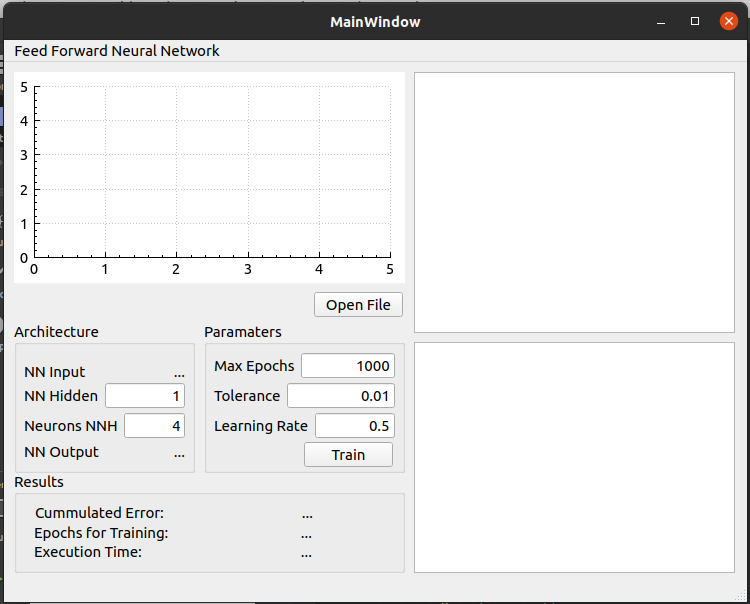
\includegraphics[width=0.7\linewidth]{interfaz}
\end{center}
Se carga el archivo para crear un dataset (se utilizó el mismo dataset de la tarea pasada).
\begin{center}
	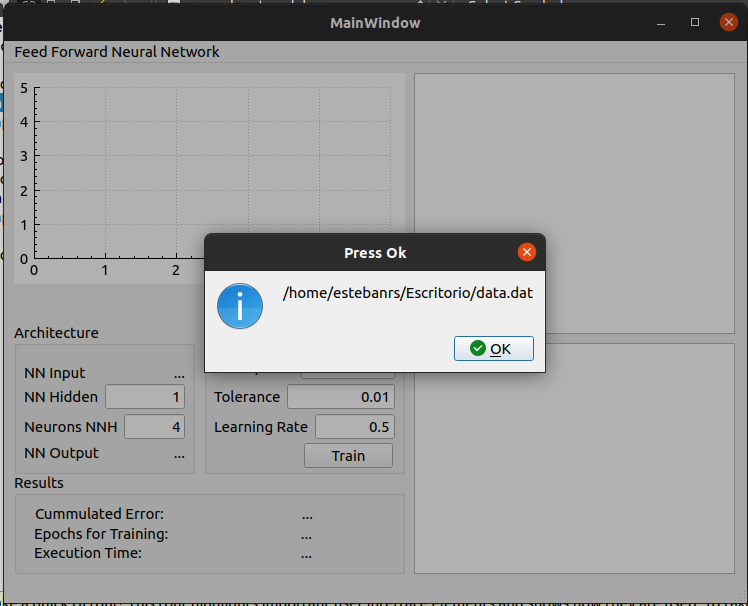
\includegraphics[width=0.7\linewidth]{archivo}
\end{center}
Tome en cuenta que si no selecciona el archivo o alguno de los parámetros no es válido, se mostará un mensaje para que revise los datos. Una vez establecidos, se pulsa el botón $ train $. A continuación se muestran tres corridas con distintos parámetros.\\
\textbf{Nota.} En la gráfica de la red neuronal, el grosor de las conexiones depende de la significancia de los pesos correspondientes.
\begin{center}
	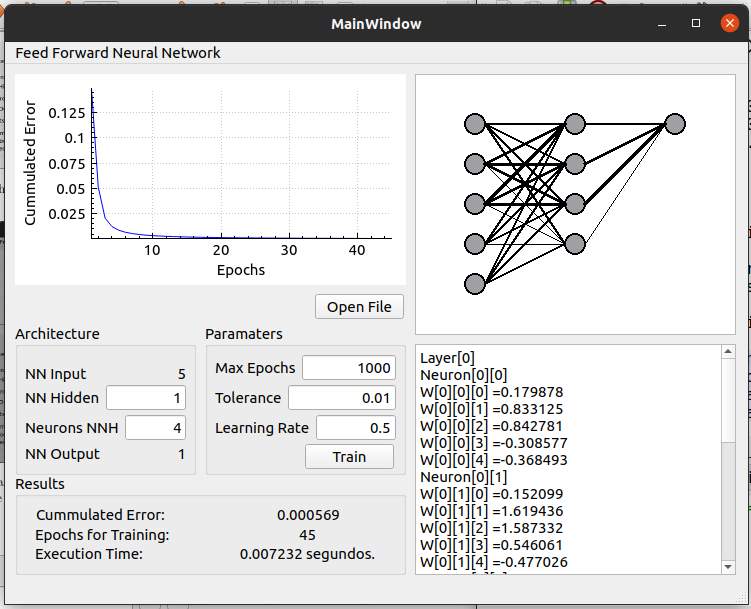
\includegraphics[width=0.7\linewidth]{1}
	\\	
	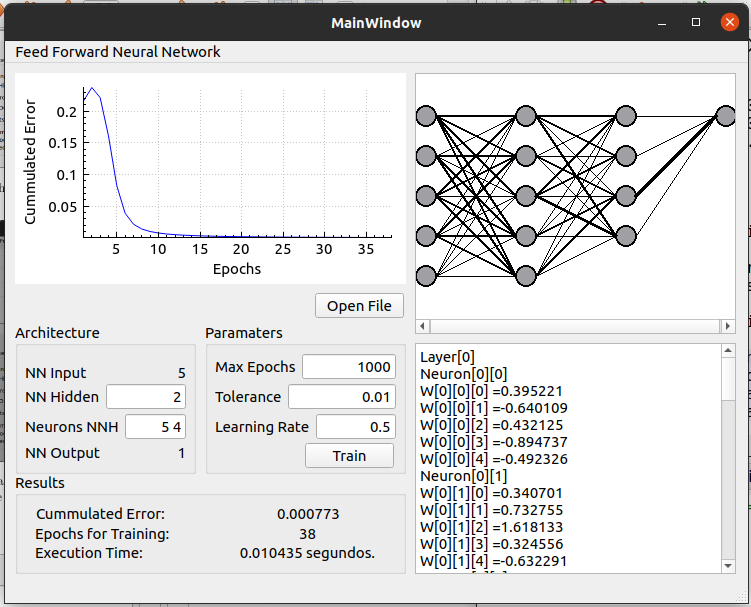
\includegraphics[width=0.7\linewidth]{2}
	\\
	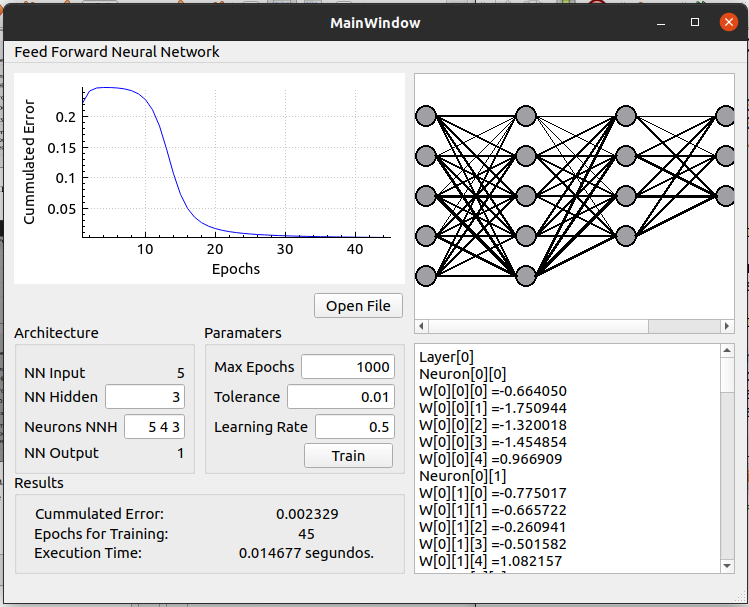
\includegraphics[width=0.7\linewidth]{3}
\end{center}

\section{Conclusiones}
Para esta base de datos la red neuronal aprendió en menos de 50 iteraciones para los parámetros establecidos y distintas arquitecturas. Esto se debe a que son pocos datos de entrenamiento y la primer columna es binaria.\\
La visualización de la curva de error permite visualizar cómo decae el error a través de las épocas y el gráfico permite ver qué pesos tienen más significancia en la red.\\
Se observa además que para una tolerancia de $ 0.0001 $ la red no converge respecto al error, esto podría deberse a que la función de error se estancó en un mínimo local.
\end{document}
